\definecolor{abink}{HTML}{20252A}
\definecolor{abblue}{HTML}{356FA8}
\definecolor{aborange}{HTML}{C47A36}
\definecolor{abred}{HTML}{B44747}
\definecolor{abpurple}{HTML}{7658A5}

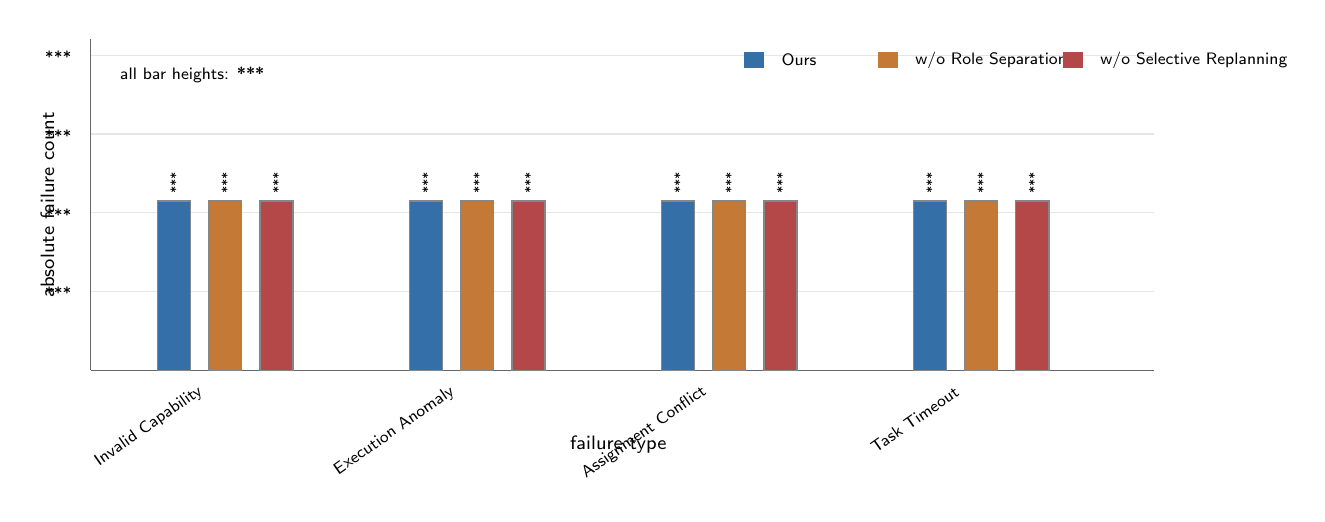
\begin{tikzpicture}[
  x=1cm,y=1cm,
  font=\sffamily\fontsize{7}{7.8}\selectfont,
  axis/.style={draw=abink!70,line width=.5pt},
  tick/.style={font=\sffamily\fontsize{6}{6.8}\selectfont},
  bar/.style={draw=abink!55,line width=.45pt},
  method/.style={font=\sffamily\fontsize{6.4}{7.2}\selectfont}
]
  \draw[axis] (0,0)--(13.5,0);
  \draw[axis] (0,0)--(0,4.2);
  \node[rotate=90] at (-.55,2.1) {absolute failure count};
  \node at (6.7,-.95) {failure type};
  \foreach \y in {1,2,3,4}{
    \draw[abink!12] (0,\y)--(13.5,\y);
    \node[tick,anchor=east] at (-.12,\y) {\texttt{***}};
  }
  \foreach \x/\lab in {1.5/{Invalid Capability},4.7/{Execution Anomaly},
                       7.9/{Assignment Conflict},11.1/{Task Timeout}}{
    \node[tick,rotate=35,anchor=east] at (\x,-.18) {\lab};
  }
  \foreach \x/\col/\name in {
      .85/abblue/Ours,1.50/aborange/{w/o Role Separation},
      2.15/abred/{w/o Selective Replanning}}{
    \draw[bar,fill=\col] (\x,0) rectangle ++(.42,2.15);
    \node[font=\sffamily\fontsize{5.4}{6.0}\selectfont,rotate=90]
      at (\x+.21,2.38) {\texttt{***}};
  }
  \foreach \x/\col in {4.05/abblue,4.70/aborange,5.35/abred}{
    \draw[bar,fill=\col] (\x,0) rectangle ++(.42,2.15);
    \node[font=\sffamily\fontsize{5.4}{6.0}\selectfont,rotate=90]
      at (\x+.21,2.38) {\texttt{***}};
  }
  \foreach \x/\col in {7.25/abblue,7.90/aborange,8.55/abred}{
    \draw[bar,fill=\col] (\x,0) rectangle ++(.42,2.15);
    \node[font=\sffamily\fontsize{5.4}{6.0}\selectfont,rotate=90]
      at (\x+.21,2.38) {\texttt{***}};
  }
  \foreach \x/\col in {10.45/abblue,11.10/aborange,11.75/abred}{
    \draw[bar,fill=\col] (\x,0) rectangle ++(.42,2.15);
    \node[font=\sffamily\fontsize{5.4}{6.0}\selectfont,rotate=90]
      at (\x+.21,2.38) {\texttt{***}};
  }
  \draw[abblue,fill=abblue] (8.3,3.85) rectangle ++(.25,.18);
  \node[method,anchor=west] at (8.65,3.94) {Ours};
  \draw[aborange,fill=aborange] (10.0,3.85) rectangle ++(.25,.18);
  \node[method,anchor=west] at (10.35,3.94) {w/o Role Separation};
  \draw[abred,fill=abred] (12.35,3.85) rectangle ++(.25,.18);
  \node[method,anchor=west] at (12.70,3.94) {w/o Selective Replanning};
  \node[method,anchor=west] at (.25,3.75) {all bar heights: \textbf{***}};
  \path[use as bounding box] (-.8,-1.2) rectangle (14.0,4.35);
\end{tikzpicture}
